\chapter{Supplementary Material}
\label{chap:supp-material}
\centerline{\rule{149mm}{.02in}}
\vspace{2cm}

TODO: intro to section

\section{Schedule}

TODO: intro

\begin{figure}[h]
	\centering
	\makebox[\textwidth][c]{
		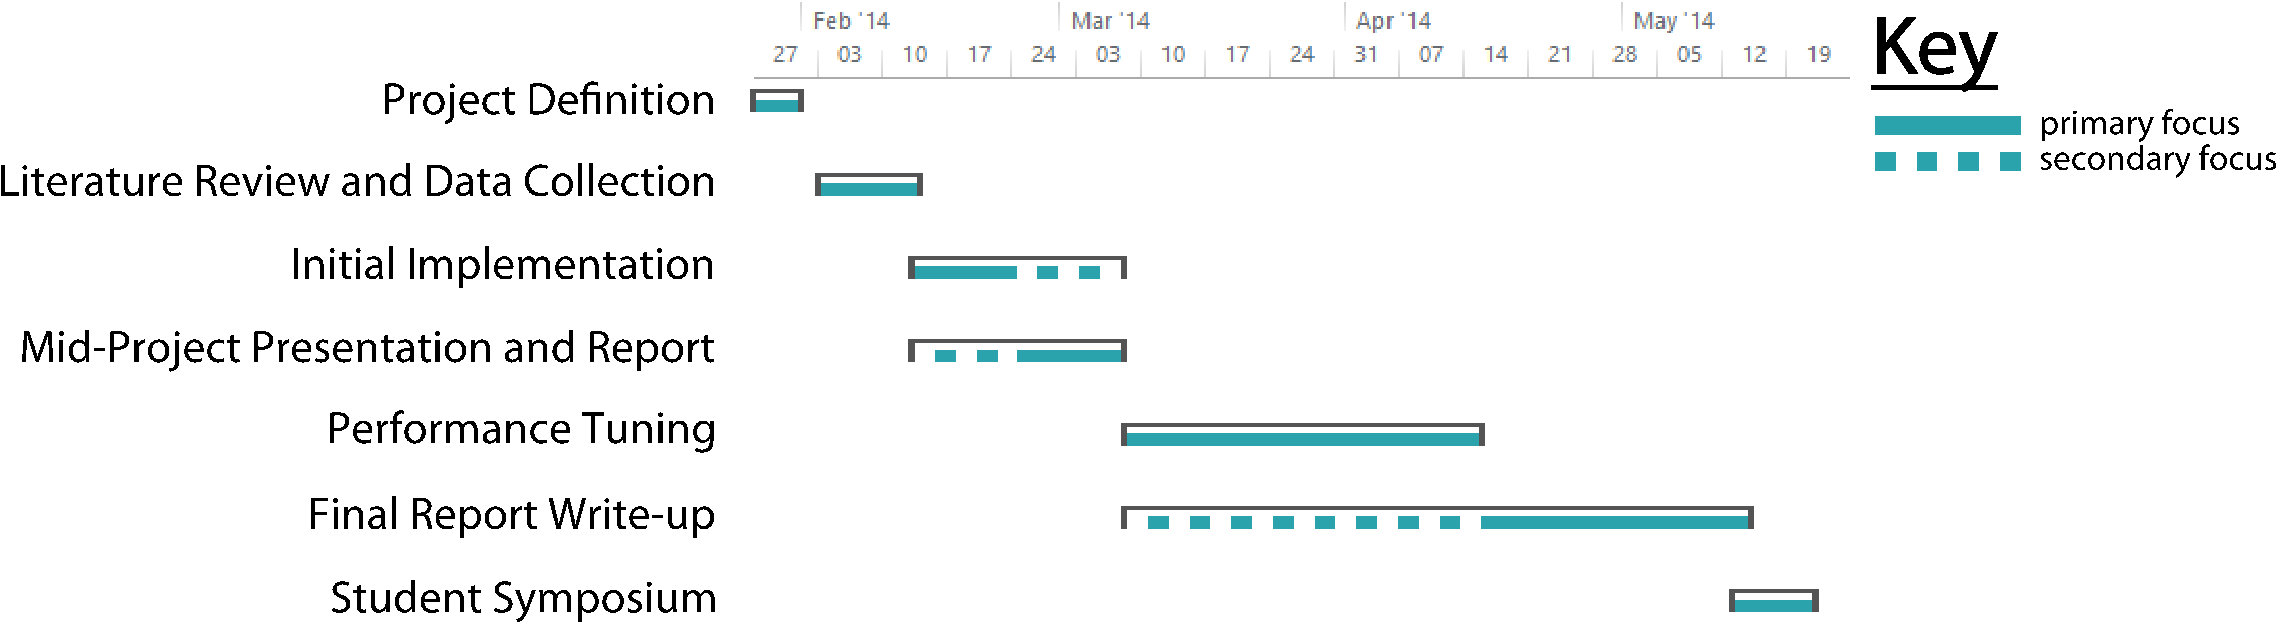
\includegraphics[scale=0.45]{figures/schedule/initial_project_schedule.pdf}
	}%
	\caption{Initial Project Schedule Created on 31/01/14}
	\label{fig:initial-schedule}
\end{figure}

\begin{figure}[h]
	\centering
	\makebox[\textwidth][c]{
		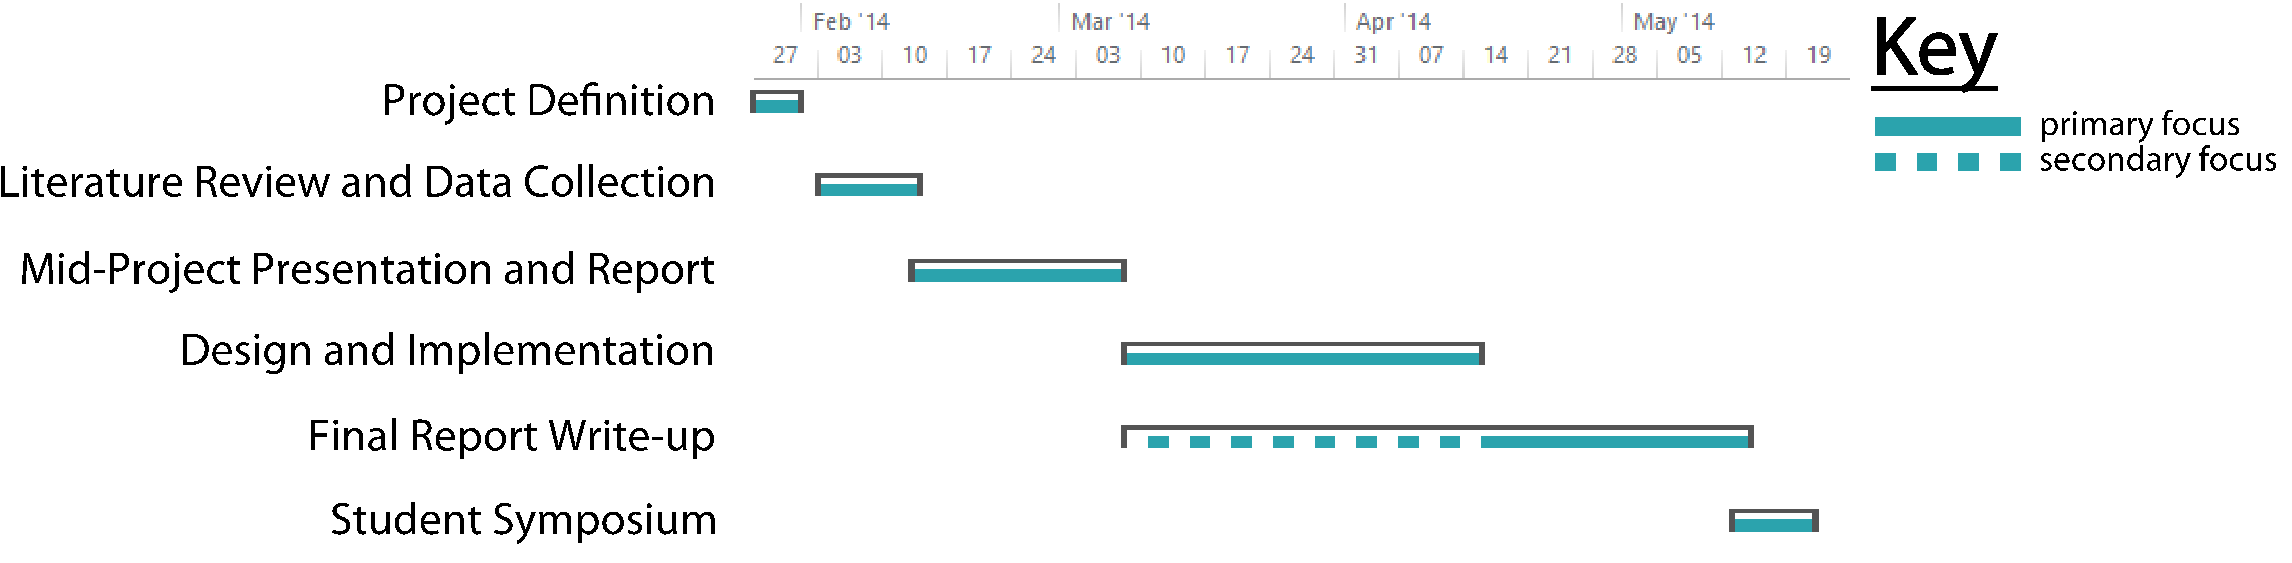
\includegraphics[scale=0.45]{figures/schedule/revised_project_schedule.pdf}
	}%
	\caption{Revised Project Schedule Created on 20/02/14}
	\label{fig:revised-schedule}
\end{figure}

\begin{figure}[h]
	\centering
	\makebox[\textwidth][c]{
		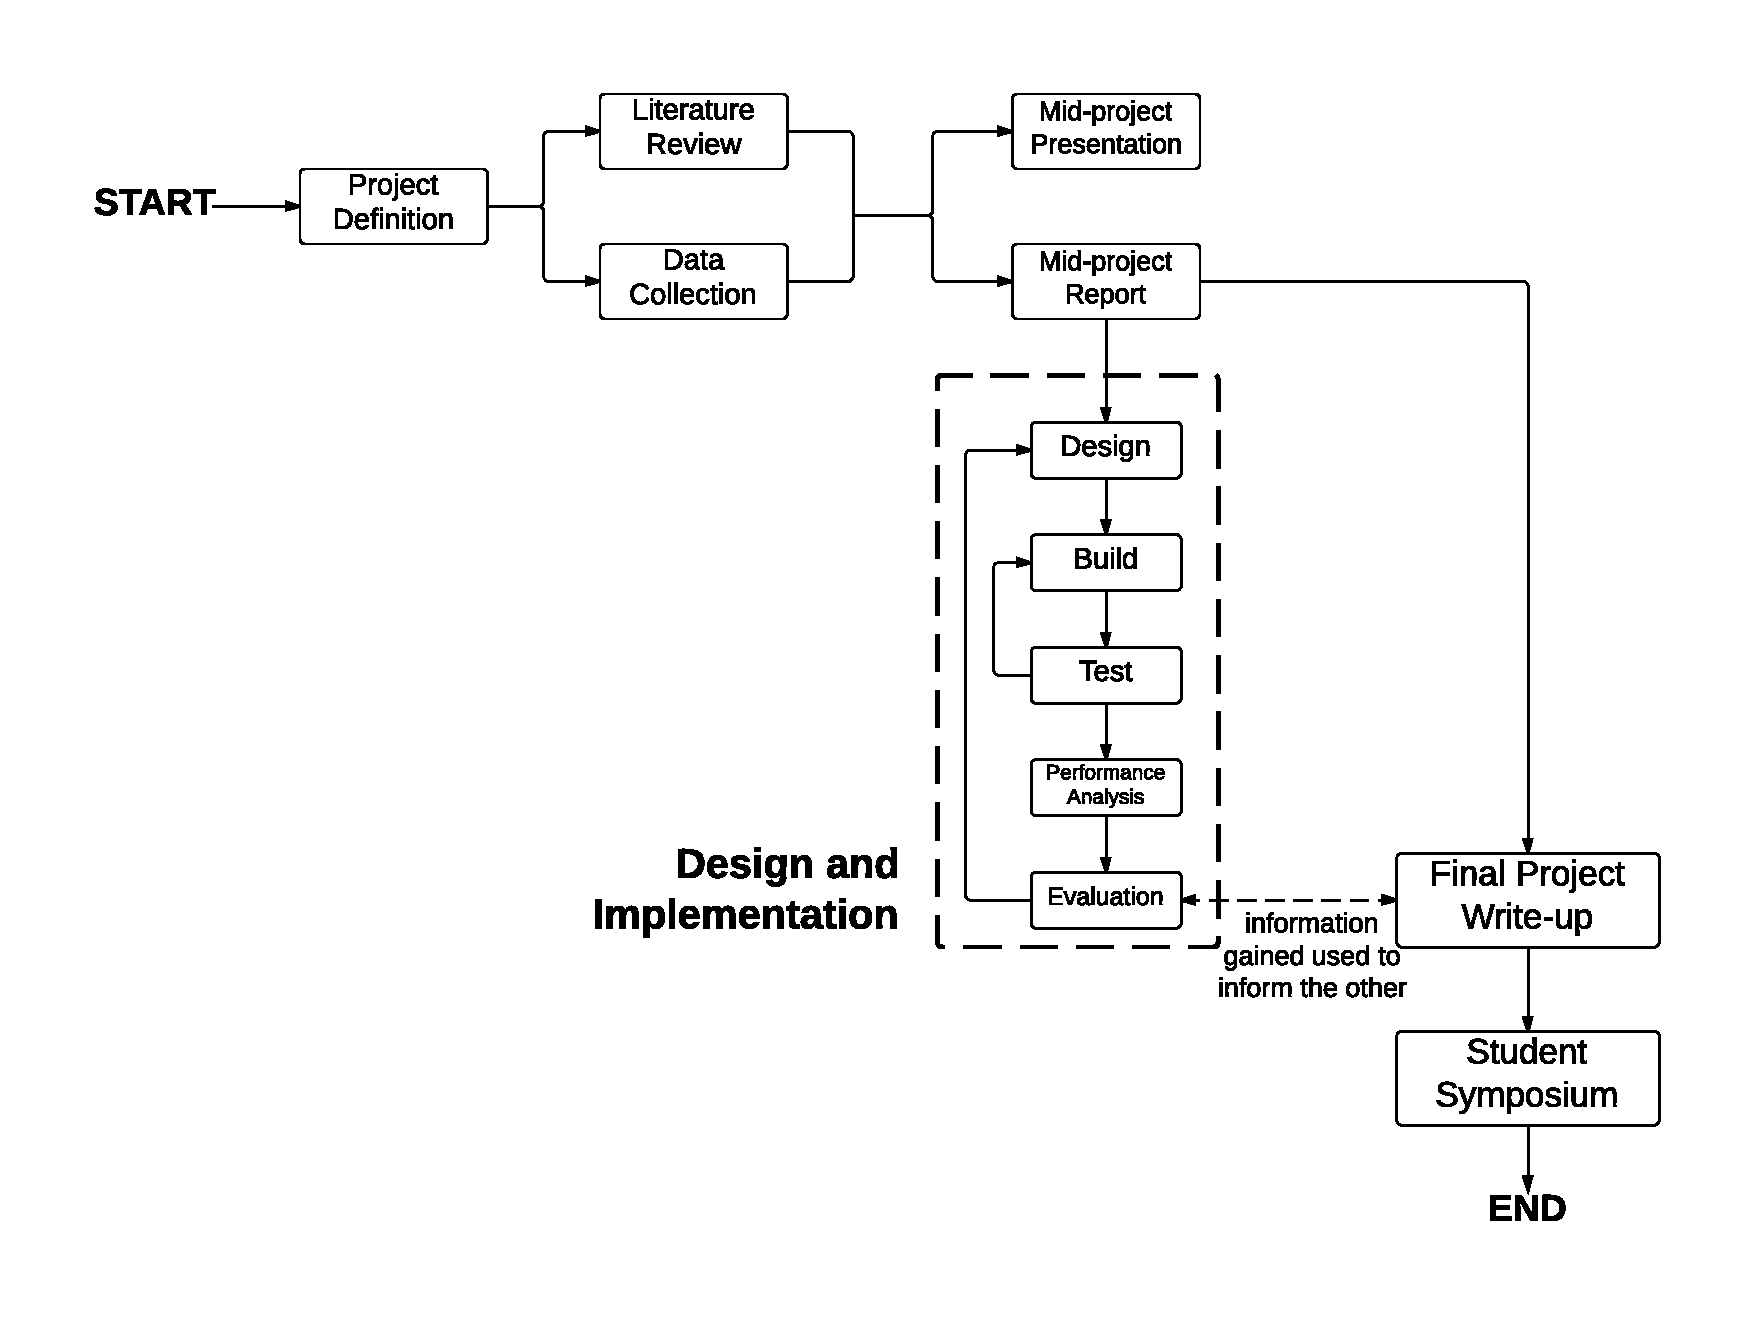
\includegraphics[scale=0.6]{figures/schedule/full-project-process.pdf}
	}%
	\caption{Flow Chart of Full Project Schedule}
	\label{fig:full-project-process}
\end{figure}

\begin{landscape}	
	\begin{figure}
		\centering
		\centerline{ 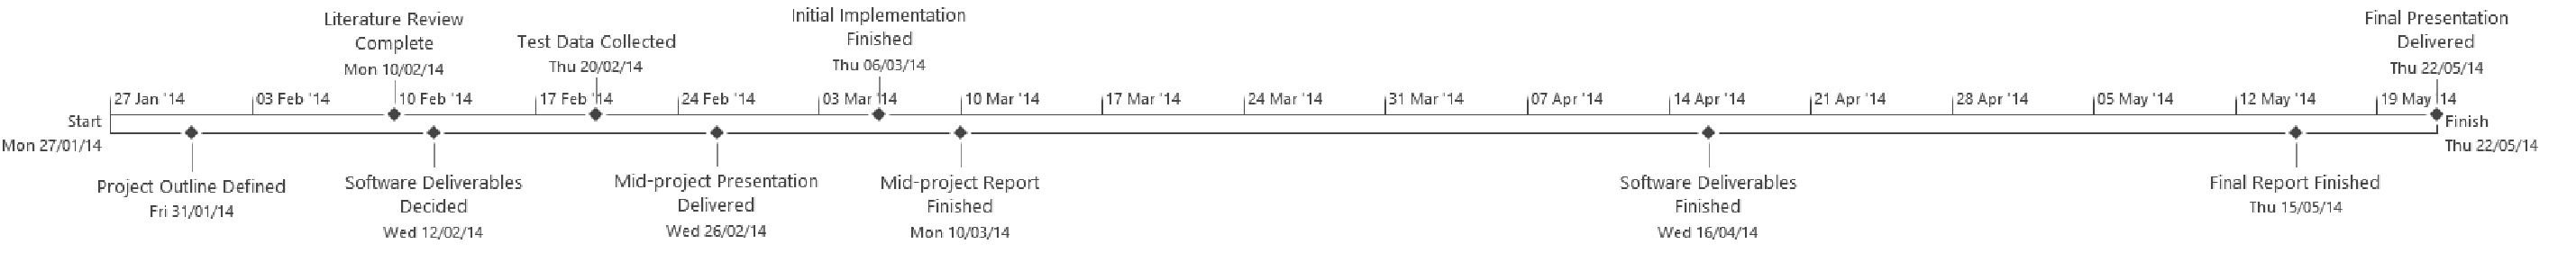
\includegraphics[scale=0.475]{figures/schedule/initial_schedule_timeline.pdf} }
		\caption{Initial Milestone Timeline Created on 20/02/14}
		\label{fig:initial-milestone-timeline}
	\end{figure}

	\begin{figure}
		\centering
		\centerline{ 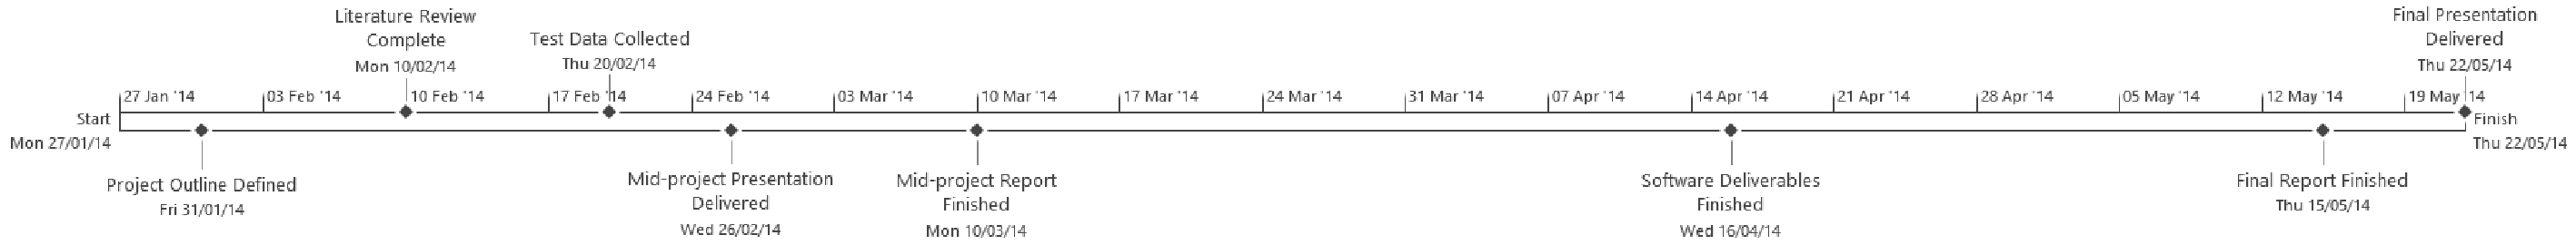
\includegraphics[scale=0.475]{figures/schedule/revised_schedule_timeline.pdf} }
		\caption{Revised Milestone Timeline Created on 20/02/14}
		\label{fig:revised-milestone-timeline}
	\end{figure}	
\end{landscape}




\begin{landscape}
	\section{Multi-dimensional Search Structures}

	TODO: intro

	\begin{table}[h]
		\centering
		\begin{tabular}{|p{2.8cm}|p{5cm}|p{5cm}|p{5cm}|p{2cm}|}
			\hline
			\textbf{Index Structure} &
			\textbf{Memory Overhead} &
			\textbf{Bucket Method?} &
			\textbf{High-Dimensional Data} &
			\textbf{Complexity} \\
			\hline
			Sequential Scan & Low & No (but since data is stored contiguously, there are minimal I/O operations due to sequential access) & Often better than other structures with high $d$ (but significantly poorer performance with low $d$) & Low \\		
			B${}^{+}$-Tree & Low & Yes & One-dimensional & Low \\
			R-Tree & Moderate & Yes & Poor for $d > 10$ \cite{pyramid-tree} & Moderate \\
			Quadtree & Low with uniformly distributed data, high for skewed data due to unnecessary nodes caused by splitting sparse regions of data space & No & Poor because it tries to use balanced splits \cite{pyramid-tree} & Low \\
			Pyramid Tree & Low & Yes (based on B${}^{+}$-tree) & Good & High \\
			PK-Tree & Moderate & No (but uses similar method to reduce I/O operations) & Good & High \\
			Skip Quadtree & Moderate & No & Untested & Moderate \\
			Quadtreap & Low & No & Untested & Moderate \\
			Splay Quadtree & Moderate & No & Untested & Moderate \\
			\hline
		\end{tabular}
		\caption{Comparison of Dynamic Multi-Dimensional Structures}
		\label{tab:comparison}
	\end{table}

	\null  % Empty line
	\nointerlineskip  % No skip for prev line
	\vfill
	\let\snewpage \newpage
	\let\newpage \relax
		\begin{figure}[H]
			\centering
			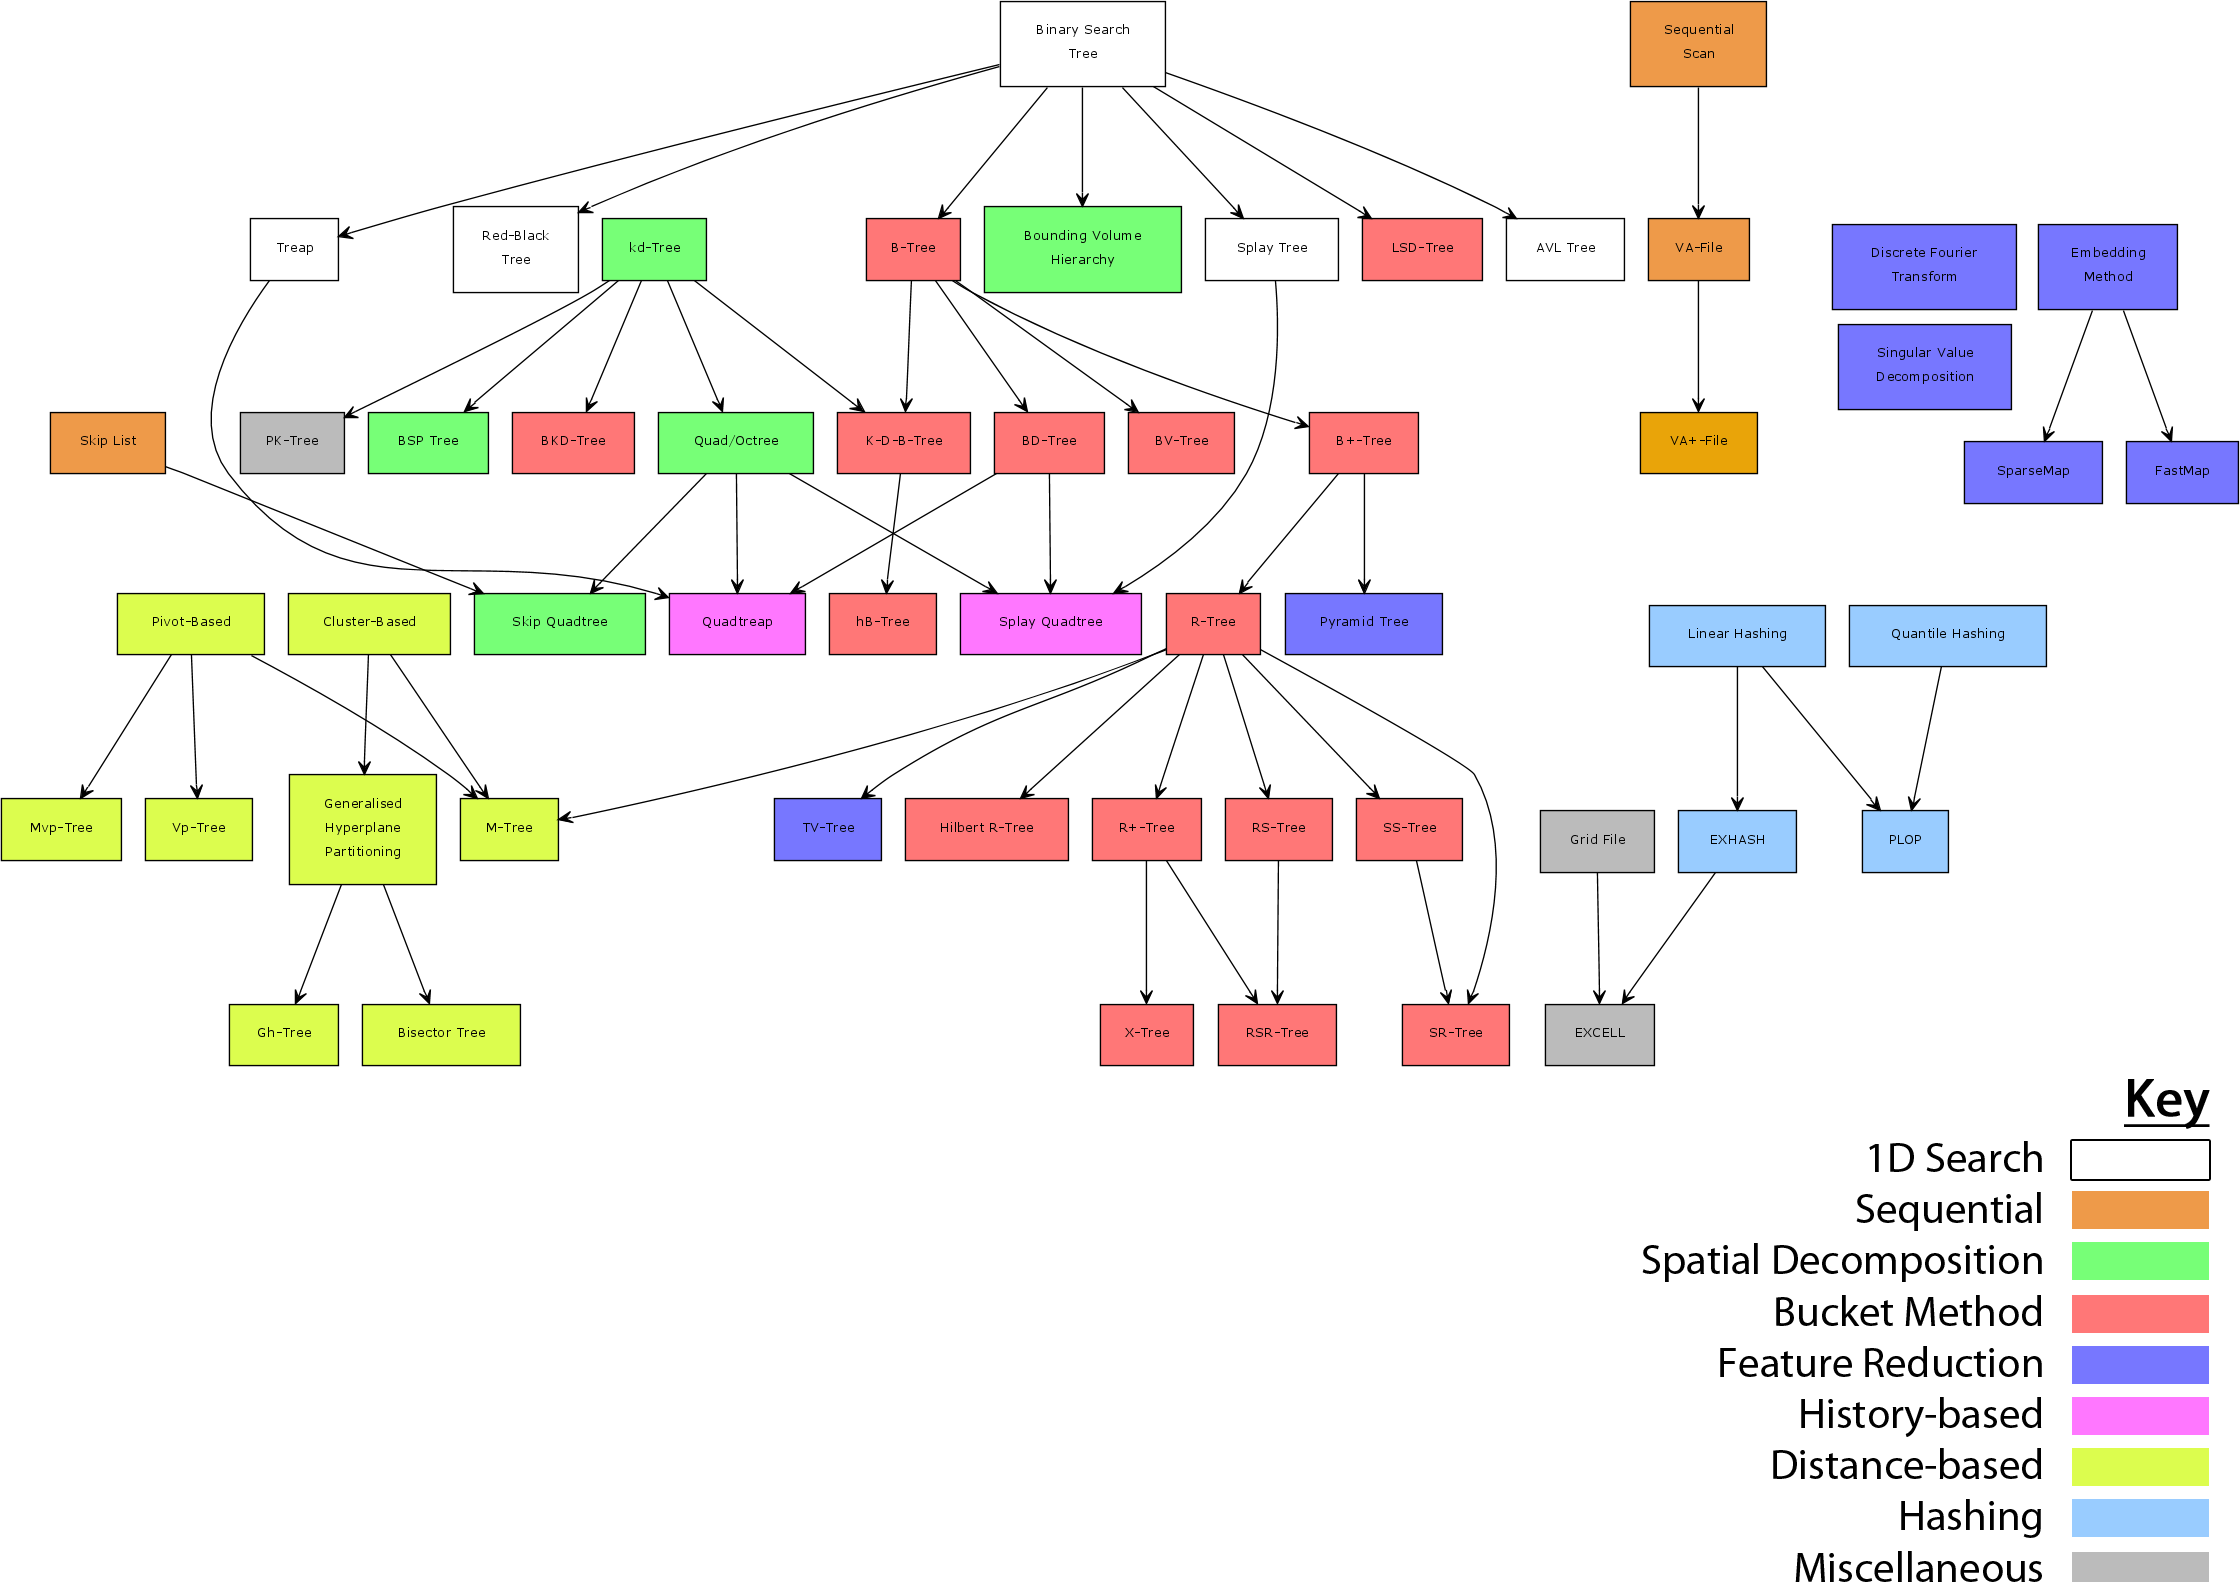
\includegraphics[scale=0.35]{figures/md_structure_taxonomy.png}
			\caption{Multi-dimensional Search Structure Taxonomy}
			\label{fig:structure-taxonomy}
		\end{figure}
	\let \newpage \snewpage
	\vfill 
	\break % page break

	\newpage

\end{landscape}




\section{Performance Timings}

TODO: intro

=ITERATION 1=
TODO: tables showing times for three operations w/ synthetic and clustered data (two tables)

=ITERATION 3=
TODO: tables showing times for three operations w/ synthetic and clustered data (two tables)




\section{Algorithms and Code Listings}

TODO: intro

\begin{algorithm}[H]
	\SetAlgoLined
	\SetKwInOut{Input}{input}\SetKwInOut{Output}{output}
	\SetKwFunction{hashPoint}{hashPoint} \SetKwFunction{hashFloat}{hashFloat}

 	\SetKwProg{funcHashPoint}{Algorithm}{}{}
  	\funcHashPoint{\hashPoint{$d, p$}} {
		\Input{$d$ = number of dimensions}
		\Input{$p_0, p_1, \dots, p_{d-1}$ = coordinates of point}
		\Output{$seed$ = integer representing hashed point}
		\Begin {
			$seed = 0$\;
			\For{$i = 0$ to $d - 1$} {
				$seed = seed \oplus \left(\hashFloat(p_i) + \texttt{0x9e3779b9} + (seed << 6) + (seed >> 2)\right)$
			}
			\KwRet{$seed$}
		}
	}

	\caption{Hashing Multi-Dimensional Point in Bucket Hash Table}
	\label{alg:point-hashing}
\end{algorithm}

\paragraph{\textbf{NOTE:}} \texttt{hashFloat} is a function which hashes an individual 32-bit floating point number and corresponds to the function \texttt{float\_hash\_impl2} in Listing \ref{lst:hash-float-function}.

\paragraph{} 

\begin{lstlisting}[label=lst:hash-float-function, caption=Code to Hash Single 32-bit Floating Point Value (Source code from file \texttt{boost/functional/hash/detail/hash\_float\_generic.hpp} in Boost Library 1.42.0)]
// Copyright 2005-2009 Daniel James.
// Distributed under the Boost Software License, Version 1.0. (See accompanying
// file LICENSE_1_0.txt or copy at http://www.boost.org/LICENSE_1_0.txt)

// A general purpose hash function for non-zero floating point values.

inline void hash_float_combine(std::size_t& seed, std::size_t value)
{
    seed ^= value + (seed<<6) + (seed>>2);
}

template <class T>
inline std::size_t float_hash_impl2(T v)
{
    boost::hash_detail::call_frexp<T> frexp;
    boost::hash_detail::call_ldexp<T> ldexp;

    int exp = 0;

    v = frexp(v, &exp);

    // A postive value is easier to hash, so combine the
    // sign with the exponent and use the absolute value.
    if(v < 0) {
        v = -v;
        exp += limits<T>::max_exponent -
            limits<T>::min_exponent;
    }

    // The result of frexp is always between 0.5 and 1, so its
    // top bit will always be 1. Subtract by 0.5 to remove that.
    v -= T(0.5);
    v = ldexp(v, limits<std::size_t>::digits + 1);
    std::size_t seed = static_cast<std::size_t>(v);
    v -= seed;

    // ceiling(digits(T) * log2(radix(T))/ digits(size_t)) - 1;
    std::size_t const length
        = (limits<T>::digits *
                boost::static_log2<limits<T>::radix>::value - 1)
        / limits<std::size_t>::digits;

    for(std::size_t i = 0; i != length; ++i)
    {
        v = ldexp(v, limits<std::size_t>::digits);
        std::size_t part = static_cast<std::size_t>(v);
        v -= part;
        hash_float_combine(seed, part);
    }

    hash_float_combine(seed, exp);

    return seed;
}
\end{lstlisting}